\chapter{Tientsin} 

\subsection{T\&S Type 1}
\begin{figure}[htbp]
\centering
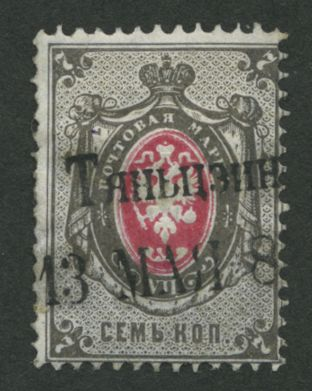
\includegraphics[width=.45\textwidth]{../russian-post-offices-in-china/10003.jpg}
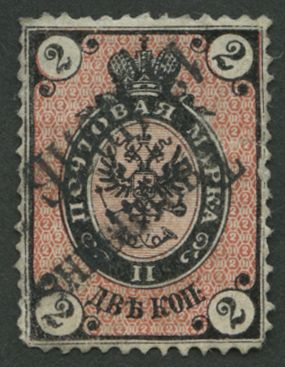
\includegraphics[width=.45\textwidth]{../russian-post-offices-in-china/10003-1.jpg}
\caption{
10003	TIENTSIN: 1879 2k and 7k with Cyrillic two-line Tientsin ds (T\&S type 1),
although its use postdates that of the type 2 cancel), minor faults, only 
three known examples of this cancel (all on loose stamps), no cover known
Note: Recorded in the British Journal of Russian Philately 71 (1991) p.8
\euro 400.00
}  
\end{figure}

\subsection{TS Type 3B}
\begin{figure}[htbp]
\centering
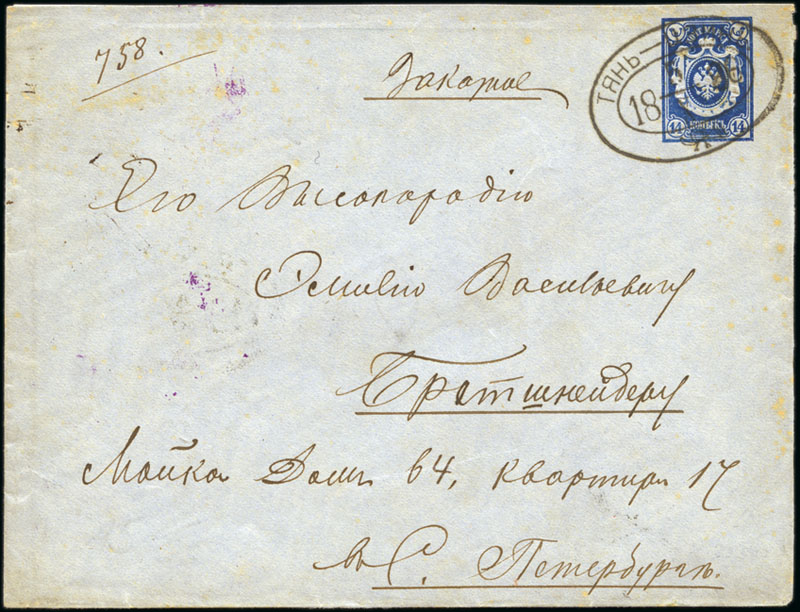
\includegraphics[width=.95\textwidth]{../russian-post-offices-in-china/10004.jpg}
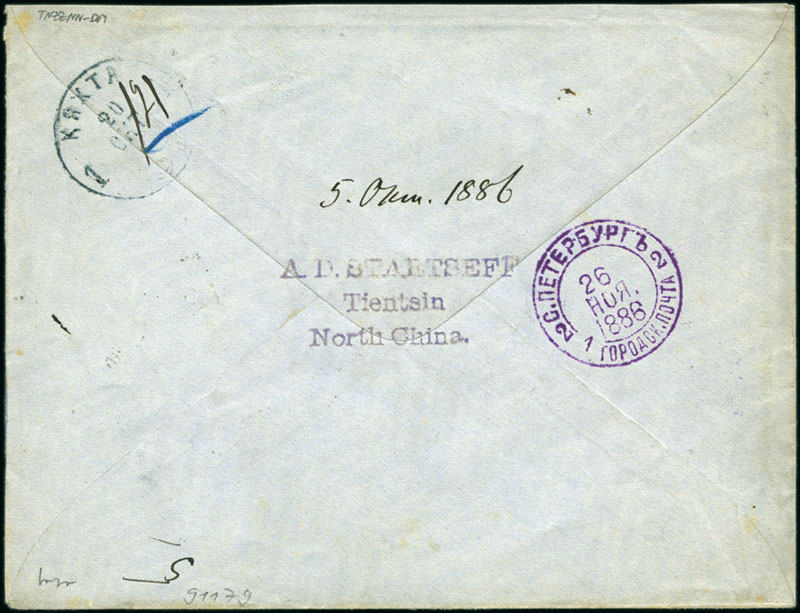
\includegraphics[width=.95\textwidth]{../russian-post-offices-in-china/10004-1.jpg}
\caption{
10004	TIENTSIN: 1886 14k Postal stationery envelope sent registered 
to St. Petersburg cancelled by double oval Tientsin 5.10.86 ds 
(T\&S type 3B, rated very scarce), with ms "Registered" (in Cyrillic)
and registered number in top left corner, with Kyakhta and St. Petersburg bs
\euro 20,000.00 
}  
\end{figure}


\begin{figure}[htbp]
\centering
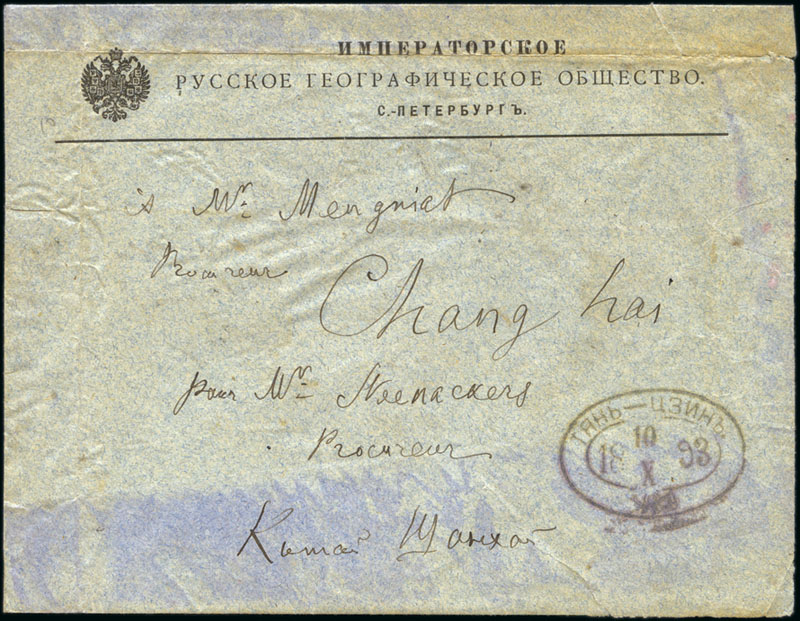
\includegraphics[width=.95\textwidth]{../russian-post-offices-in-china/10005.jpg}
\caption{
10005 TIENTSIN INCOMING: 1893 Cover from the Imperial Russian Geographical 
Society in St. Petersburg to Shanghai via the Russian P.O. in Tientsin, 
sent unfranked, with St. Petersburg, double oval Tientsin 10.10.93 (T\&S type 3B) arrival, missing a back flap and some creasing
\euro 400.00 
}  
\end{figure}

\begin{figure}[htbp]
\centering
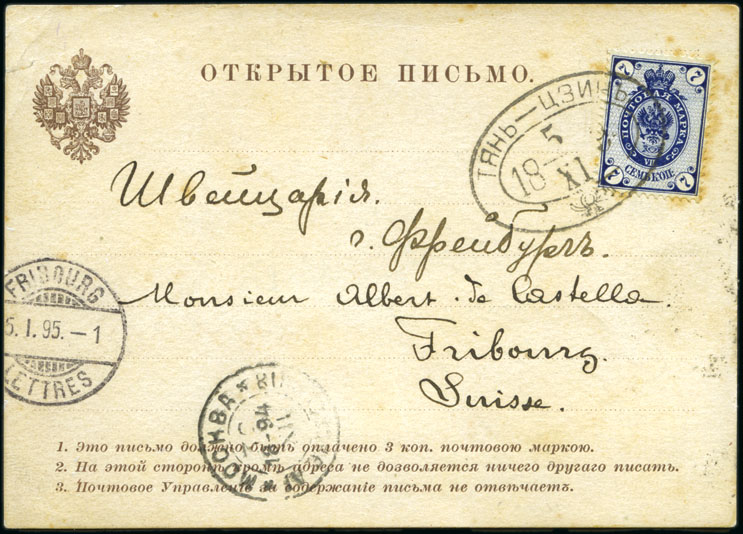
\includegraphics[width=.95\textwidth]{../russian-post-offices-in-china/10006.jpg}
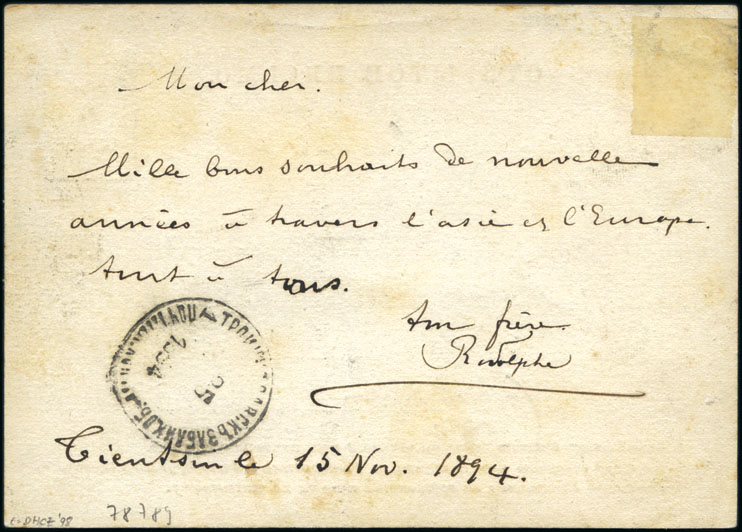
\includegraphics[width=.95\textwidth]{../russian-post-offices-in-china/10006-1.jpg}
\caption{
10006		ZoomTIENTSIN: 1894 Postcard to Switzerland with 1889-92 7k tied 
by double oval Tientsin 5.6.94 ds (T\&S type 3B), with Troitskosavsk, 
Moscow transits and Fribourg arrival, some toning around the stamp, it took 59 days 
in total incl. about 8 weeks to get to Moscow due to the deterioration of 
the postal route across the Gobi desert, Mongolia and Siberia during the 
winter, very rare
\euro 20,000.00
}  
\end{figure}











                        